\documentclass[final]{beamer} % beamer 3.10: do NOT use option hyperref={pdfpagelabels=false} !
%\documentclass[final,hyperref={pdfpagelabels=false}]{beamer} % beamer 3.07: get rid of beamer warnings
\mode<presentation> {  %% check http://www-i6.informatik.rwth-aachen.de/~dreuw/latexbeamerposter.php for examples
  \usetheme{qcv}    %% you should define your own theme e.g. for big headlines using your own logos
}
\usepackage[english]{babel}
\usepackage[latin1]{inputenc}
\usepackage{fancyvrb}
\usepackage{wrapfig}
\usepackage{amsmath,amsthm, amssymb, latexsym}
%\usepackage{times}\usefonttheme{professionalfonts}  % times is obsolete
\usefonttheme[onlymath]{serif}
\boldmath
\usepackage[orientation=landscape,size=a0,scale=1.4]{beamerposter}                       % e.g. for DIN-A0 poster
%\usepackage[orientation=landscape,size=a0,scale=1.4,debug]{beamerposter}                       % e.g. for DIN-A0 poster
%\usepackage[orientation=portrait,size=a1,scale=1.4,grid,debug]{beamerposter}                  % e.g. for DIN-A1 poster, with optional grid and debug output
%\usepackage[size=custom,width=200,height=120,scale=2,debug]{beamerposter}                     % e.g. for custom size poster
%\usepackage[orientation=portrait,size=a0,scale=1.0,printer=rwth-glossy-uv.df]{beamerposter}   % e.g. for DIN-A0 poster with rwth-glossy-uv printer check

\title[QCViewer]{QCViewer}
\author[Author]{Alex Parent, Jacob Parker, Marc Burns and Dmitri Maslov}
\institute[IQC, University of Waterloo]{Quantum Circuits group, IQC, University of Waterloo}
\date{\today}


\begin{document}
    \begin{frame}{}
    \begin{columns}
        \begin{column}{.33\textwidth}
        \begin{beamercolorbox}[center,wd=\textwidth]{postercolumn}
        \begin{minipage}[c][0.95\textheight][s]{0.95\columnwidth}
            % Overview Section
            \begin{block}{\large Overview}
              QCViewer is a tool for displaying, editing, and simulating
              quantum circuits. It allows users to test new circuit designs
              and make publication quality diagrams with an easy-to-use
              graphical interface.

                Features include: % XXX mention unitary stuff?
                \begin{itemize}[]
                    \item A rich language for specifying quantum circuits
                    \item Interactive drag-and-drop circuit layout
                    \item Circuit simulation
                    \item \LaTeX\hspace{0.5em}integration and offline rendering
                    \item Vector graphics format (SVG) output
                \end{itemize}

                \begin{center}
                    \includegraphics{figures/QCViewerGUI.png}
                \end{center}
            \end{block}
            \vfill
            % Motivation Section
            \begin{block}{\large Motivation}
                Our goal in developing \textcolor{blue}{QCViewer} is to provide
                a convenient tool that is useful to the quantum computing
                community for both research and educational purposes.
                QCViewer provides a drag and drop interface for circuit design.
                This makes it easy to quickly test out new algorithms and circuit design ideas.
                In order to make the diagrams useful for presentation (e.g.
                Adobe Illustrator, PowerPoint) and publication (e.g. \LaTeX),
                we provide the ability to export images in SVG, PNG, and EPS formats.
                \begin{center}
                    \includegraphics[height=6.20in]{figures/Motivation.png}
                \end{center}
            \end{block}
        \end{minipage}
        \end{beamercolorbox}
        \end{column}

        \begin{column}{.33\textwidth}
        \begin{beamercolorbox}[center,wd=\textwidth]{postercolumn}
        \begin{minipage}[c][0.95\textheight][s]{0.95\columnwidth}
            % Circuit Design Section
            \begin{block}{\large Circuit Design}

                QCViewer stores circuits in a quantum circuit description
                language called ``.qc''.  Circuits can be designed
                interactively in QCViewer or by writing a text
                description of the circuit. Other software tools can easily be
                adapted to output this format; QCViewer can then be used to
                visualize and simulate the circuits output by these tools.
                \begin{figure}[!htbp]
                \centering
                \begin{minipage}{0.9\textwidth}
                  \hspace{1em}
                  \begin{wrapfigure}{r}{0.7\textwidth}
                    \vspace*{1.5em}
                    \begin{center}
                      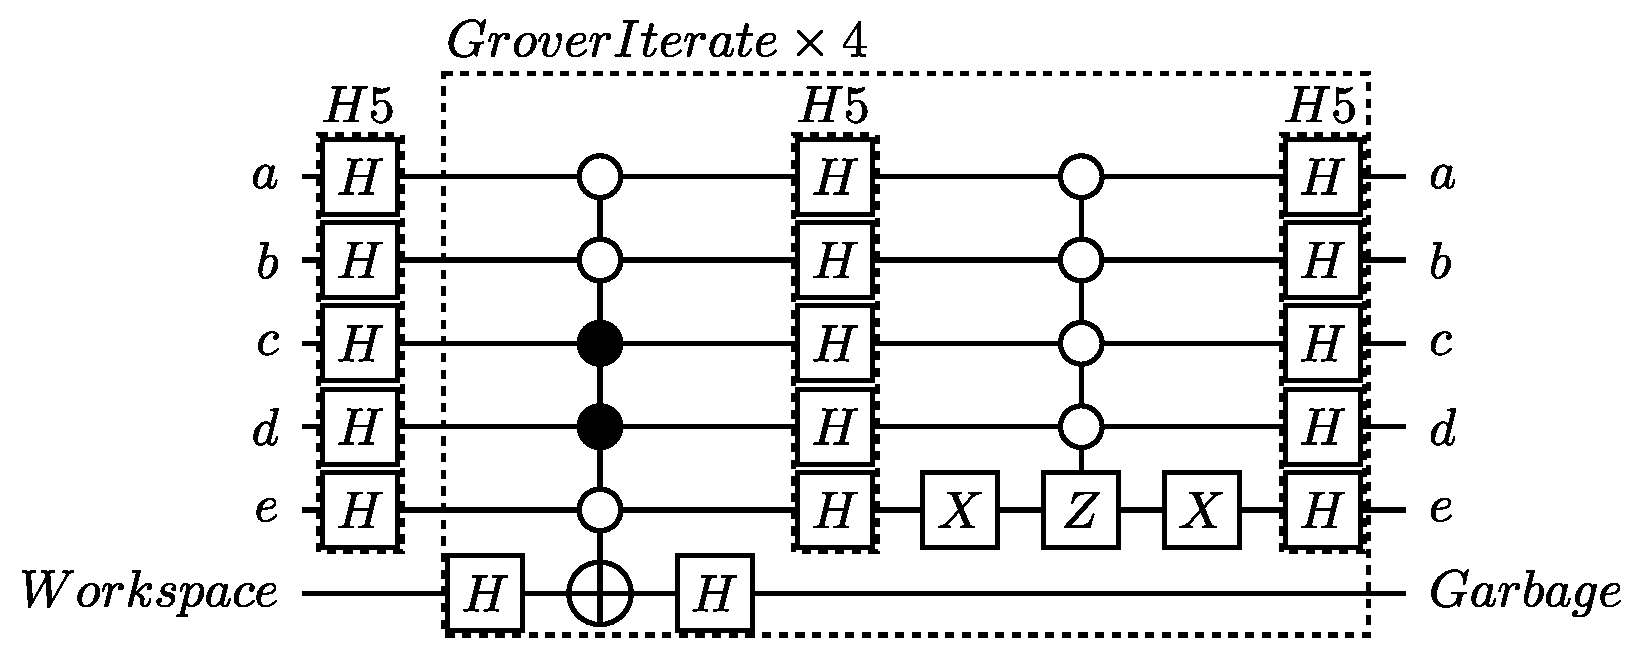
\includegraphics[height=3in]{figures/Grover_Circuit.eps}
                    \end{center}
                  \end{wrapfigure}
                  \hrule
                  \VerbatimInput[fontsize=\fontsize{12pt}{12pt}]{grover.qc}
                  \hrule
                  \vspace*{1em}
                \end{minipage}
                \caption{The ``.qc'' description and corresponding graphical representation of Grover's circuit.}
                \end{figure}

                The text on the left corresponds to a ``.qc'' specification of the circuit on the right.
                Circuit inputs and outputs $\ell_1, \ldots, \ell_n$ are specified in the header.
                The user describes a circuit block as a series of gates and sub-circuits between a pair of ``BEGIN'' and ``END'' tags.
                The grammar for this description is given below, where $w_1 \ldots w_n$ denotes a mixed list of controls and targets
                corresponding to the named gate.

                \vspace*{1em}
                \begin{tabular}{lrl}
                  $input$ & $:=$ & $header$ $input$\\
                          & $|$  & {\tt START} CircuitName {\tt (} $w_1 \ldots w_n$ {\tt )}
                                 $gates$ {\tt END} $input$\\
                          & $|$  & {\tt START} $gates$ {\tt END} $input$\\
                  $gates$ & $:=$ & $gate$ $gates$\\
                  $gate$  & $:=$ & $gatespec$ $w_1 \ldots w_n$\\
                          & $|$  & $gatespec$ {\tt (} $\theta$ {\tt )} $w_1$ \hspace{7em}{\it\small Rotation by $\theta$}\\
                          & $|$  & $gatespec$ {\tt (} $k$ {\tt pi /} $j$ {\tt )} $w_1$ \hspace{3.5em}{\it\small Rotation by $\frac{k\pi}{j}$}\\
                  $gatespec$
                          & $:=$ & GateName\\
                          & $|$  & GateName{\tt\textasciicircum}$p$ \hspace{10em}{\it\small Looping $p$ times}\\
                  $w$     & $:=$ & $\ell$ $|$ $\ell${\tt{'}} \hspace{10em}{\it\small {\tt{'}} denotes control inversion}
                \end{tabular}
                \vspace*{1em}

		        \begin{figure}[!htbp]
		            \centering
		            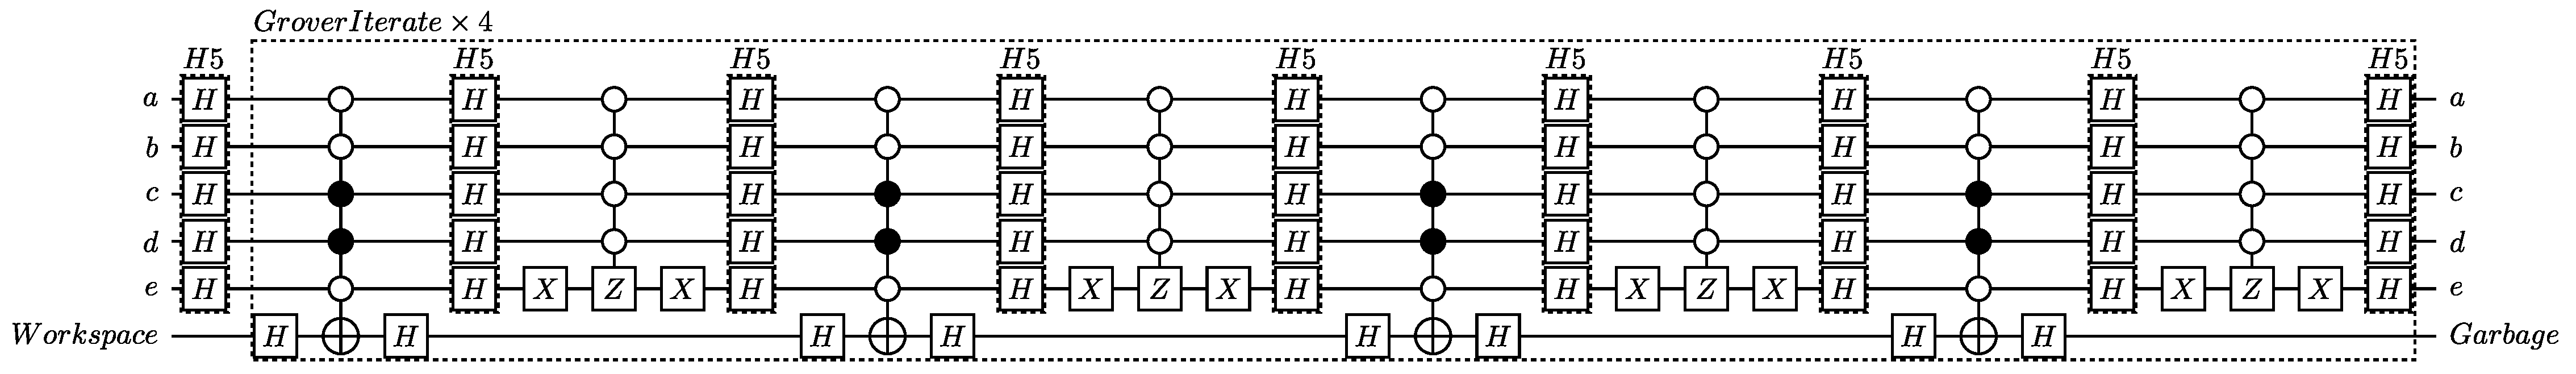
\includegraphics[width=\textwidth]{figures/Grover_Unrolled.eps}
		            \caption{Grover's circuit with iterations and sub-circuits unrolled.}
		        \end{figure}
            \end{block}
            \vfill
            % References Section
            \begin{block}{\large References}
		    \begin{thebibliography}{9}
                \small{
		            \bibitem{NC00}
  		            M.A. Nielsen and I. L. Chuang,
  		            \emph{Quantum Computation and Quantum Information}.
  		            Cambridge University Press,
		            Cambridge New York,
  		            2000.
                }
		    \end{thebibliography}
            \end{block}
            \vfill
        \end{minipage}
        \end{beamercolorbox}
        \end{column}

        \begin{column}{.33\textwidth}
        \begin{beamercolorbox}[center,wd=\textwidth]{postercolumn}
        \begin{minipage}[c][0.95\textheight][s]{0.95\columnwidth}
            % Circuit Simulation Section
            \begin{block}{\large Circuit Simulation}
                Simulation is done using a sparse state vector.
                This allows some circuits,
                such as reversible circuits with classical inputs,
                to be simulated efficiently.

                Features include breakpoints, step by step simulation, and graphical display.
		        \begin{figure}[!htbp]
		            \centering
		            \includegraphics[width=\textwidth]{figures/state.png}
		            \caption{Grover circuit and corresponding text.}
		        \end{figure}
                The circuit simulator can display graphs of the probability
                distribution, real amplitudes, or imaginary amplitudes of the
                state in the computational basis.
                \vspace*{0.5em}
            \begin{figure}[!htbp]
		            \centering
		            \includegraphics[width=0.49\textwidth]{figures/Grover_Simulate1.png} \ \  \includegraphics[width=0.49\textwidth]{figures/Grover_Simulate2.png}
		            \caption{Grover circuit and corresponding text.}
		        \end{figure}
            \end{block}
            \vfill
            \begin{block}{\large Software}
                You can download a copy of QCViewer from: \texttt{http://qcirc.iqc.uwaterloo.ca}.
            \end{block}
            \vfill
            % Acknowledgments Section
            % XXX get vector graphics
            % XXX add IARPA and TORQUE
            \begin{block}{\large Acknowledgments}
                This work has been supported in part by the IARPA and TORQUE project.
                \begin{center}
                    \includegraphics[height=1.5in]{figures/torque.png} \\ \includegraphics[height=2in]{figures/iarpa_logo.png}
                \end{center}
            \end{block}
        \end{minipage}
        \end{beamercolorbox}
        \end{column}
    \end{columns}
    \end{frame}
\end{document}
